\usepackage[b5paper, top=10mm, text={144mm, 208mm}, includehead, includefoot, hmarginratio=1:1, heightrounded]{geometry}
	\pdfpagewidth=176truemm
	\pdfpageheight=250truemm
\usepackage[explicit,clearempty]{titlesec}
\usepackage{wallpaper,changepage,fancyhdr,tikz,indentfirst}
\usepackage{amssymb,amsfonts,amsmath,amsthm,bm,mathrsfs}
\def\pgfsysdriver{pgfsys-dvipdfm.def}
\usepackage[all]{xy}
\usetikzlibrary{shapes,positioning}
\usepackage{hyperref}
	\hypersetup{bookmarksnumbered=true}

%% Define how the chapter title is printed
\titleformat{\chapter}{}{}{0pt}{
%% Background image at top of page
%% Draw a semi-transparent rectangle across the top
	%% Check if on an odd or even page
	\strictpagecheck\checkoddpage
	\ifoddpage{
	}
	\else {
		\newpage
		\thispagestyle{plain}
	}
	\fi
	\tikz[overlay,remember picture]
	\fill[opacity=.7]
	(current page.north west) rectangle 
	([yshift=-3cm] current page.north east);
	\begin{tikzpicture}[overlay,remember picture]
	\node[anchor=south west,text=white,
		xshift=20mm,yshift=-25mm,
		font=\sffamily\bfseries\huge] 
		at (current page.north west) 
		{\chaptername\ \thechapter};
	\node[fill=Sienna!80!black,text=white,
		font=\Huge\bfseries, 
		inner ysep=12pt, inner xsep=20pt,
		rounded rectangle,anchor=east, 
		xshift=-20mm,yshift=-30mm] 
		at (current page.north east) {#1};
	\end{tikzpicture}
}
%% Define how the chapter title is printed
\titleformat{name=\chapter,numberless}{}{}{0pt}{
%% Draw a semi-transparent rectangle across the top
\tikz[overlay,remember picture]
	\fill[opacity=.7]
	(current page.north west) rectangle 
	([yshift=-3cm] current page.north east);
	\begin{tikzpicture}[overlay,remember picture]
	\node[fill=Sienna!80!black,text=white,
		font=\Huge\bfseries, 
		inner ysep=12pt, inner xsep=20pt,
		rounded rectangle,anchor=east, 
		xshift=-20mm,yshift=-30mm] 
		at (current page.north east) {#1};
	\end{tikzpicture}
}
\titlespacing*{\chapter}{0pt}{0pt}{100mm}
\titlespacing*{name=\chapter,numberless}{0pt}{0pt}{50mm}

%% Set the uniform width of the colour box
%% displaying the page number in footer
%% to the width of "99"
\newlength\pagenumwidth
\settowidth{\pagenumwidth}{99}

%% Define style of page number colour box
\tikzset{pagefooter/.style={
anchor=base,font=\sffamily\bfseries\small,
text centered,text depth=17mm,text width=\pagenumwidth}}

%% Concoct some colours of our own
\definecolor[named]{GreenTea}{HTML}{000000}

%%%%%%%%%%
%%% Re-define running headers on non-chapter pages
%%%%%%%%%%
\fancypagestyle{headings}{%
	\fancyhf{}   % Clear all headers and footers first
	%% Right headers on odd pages
	\fancyhead[RO]{%
	%% First draw the background rectangles
	%% Then the decorative line and the right mark
	
\begin{tikzpicture}[xshift=-.75\baselineskip,yshift=.25\baselineskip,remember picture,    overlay,fill=GreenTea,draw=GreenTea]\fill circle(3pt);\draw[semithick](0,0) -- (current page.west |- 0,0);\end{tikzpicture} \sffamily\itshape\small\nouppercase{\rightmark}
	}

	%% Left headers on even pages
	\fancyhead[LE]{%
	%% Background rectangles first
	%% Then the right mark and the decorative line
	\sffamily\itshape\small\nouppercase{\leftmark}\ 
	\begin{tikzpicture}[xshift=.5\baselineskip,yshift=.25\baselineskip,remember picture, overlay,fill=GreenTea,draw=GreenTea]\fill (0,0) circle (3pt); \draw[semithick](0,0) -- (current page.east |- 0,0 );\end{tikzpicture}
	}

	%% Right footers on odd pages and left footers on even pages,
	%% display the page number in a colour box
	\fancyfoot[RO,LE]{\tikz[baseline]\node[pagefooter]{\thepage};}
	\renewcommand{\headrulewidth}{0pt}
	\renewcommand{\footrulewidth}{0pt}
}

%%%%%%%%%%
%%% Re-define running headers on chapter pages
%%%%%%%%%%
\fancypagestyle{plain}{%
	%% Clear all headers and footers
	\fancyhf{}
	%% Right footers on odd pages and left footers on even pages,
	%% display the page number in a colour box
	\fancyfoot[RO,LE]{\tikz[baseline]\node[pagefooter]{\thepage};}
	\renewcommand{\headrulewidth}{0pt}
	\renewcommand{\footrulewidth}{0pt}
}